%!TEX root = /Users/stevenmartell/Documents/CURRENT PROJECTS/iSCAM-trunk/fba/BC-herring-2011/WRITEUP/BCHerring2011.tex


\section{Introduction}

The objectives of this section of the report are: (1) present the data used in the 2011 assessment, (2) provide a summary overview of the integrated statistical catch-age model (hereafter, \iscam), (3) present the 2011 stock assessment and forecast for 2012, and (4) describe in detail the decision table used to provide advice to fisheries management.

BC herring are currently managed as five major stocks and 2 minor stocks (Figure \ref{Fig1}).  Annual catch advice for each of these areas is based on current estimates of stock status, and a 20\% exploitation rate if the stock is above the cutoff level for the five major stocks and a 10\% exploitation rate for the two minor stocks.  Cutoff levels for the five major stocks are based on 0.25$B_o$, and estimates of unfished biomass were established first in 1985 \citep{haist1986stock}.  These cutoffs are currently are thought to be more conservative 	than the current default Limit Reference Point of 0.4\bmsy\ \citep{dfo2006}.  Alternative cutoffs based on updated estimates of $B_o$ are also provided in this document.

This years assessment is based on a new model, \iscam, where alternative assumptions about survey $q$, and the form of the error distribution for the age-composition data are the major differences in comparison to the 2010 assessment using HCAM.



\section{BC Herring Stocks}
The geographic boundaries used to delineate the B.C. herring stock assessment regions have remained consistent since 1993.  Boundaries and locations of the major stock and minor stock areas are identified in Figure \ref{II:fig:map}.  The Haida Gwaii (HG) or Queen Charlotte Islands (QCI2E) stock assessment region includes most of Statistical Area 2E, spanning from Cumshewa Inlet in the north to Louscoone Inlet in the south.  The Prince Rupert District (PRD) stock assessment region encompasses Statistical Areas 03 to 05.  The Central Coast (CC) assessment region separates the major migratory stocks from the minor spawning populations in the mainland inlets.  The Central Coast assessment region includes Statistical Area 07 plus Kitasu Bay in Area 06, Kwakshua Channel in Section 085 and Fitz Hugh Sound in Section 086.  The Strait of Georgia (SOG) stock assessment region includes all of Statistical Areas 14 to 19, 28, and 29 (excluding Section 293), Deepwater Bay and Okisollo Channel, both in Section 132, and Section 135.  The west coast of Vancouver Island (WCVI) assessment region encompasses Statistical Areas 23 to 25.  The minor stocks include all of Area 27 and Area 2W (excluding Louscoone Inlet in Section 006).  Current geographic stock boundaries are outlined in \cite{Midgley:2003fk}, although note that SOG sections 280 and 291 do not appear as they were added in 2006.

\begin{figure}[!tbp]
	% Requires \usepackage{graphicx}
	%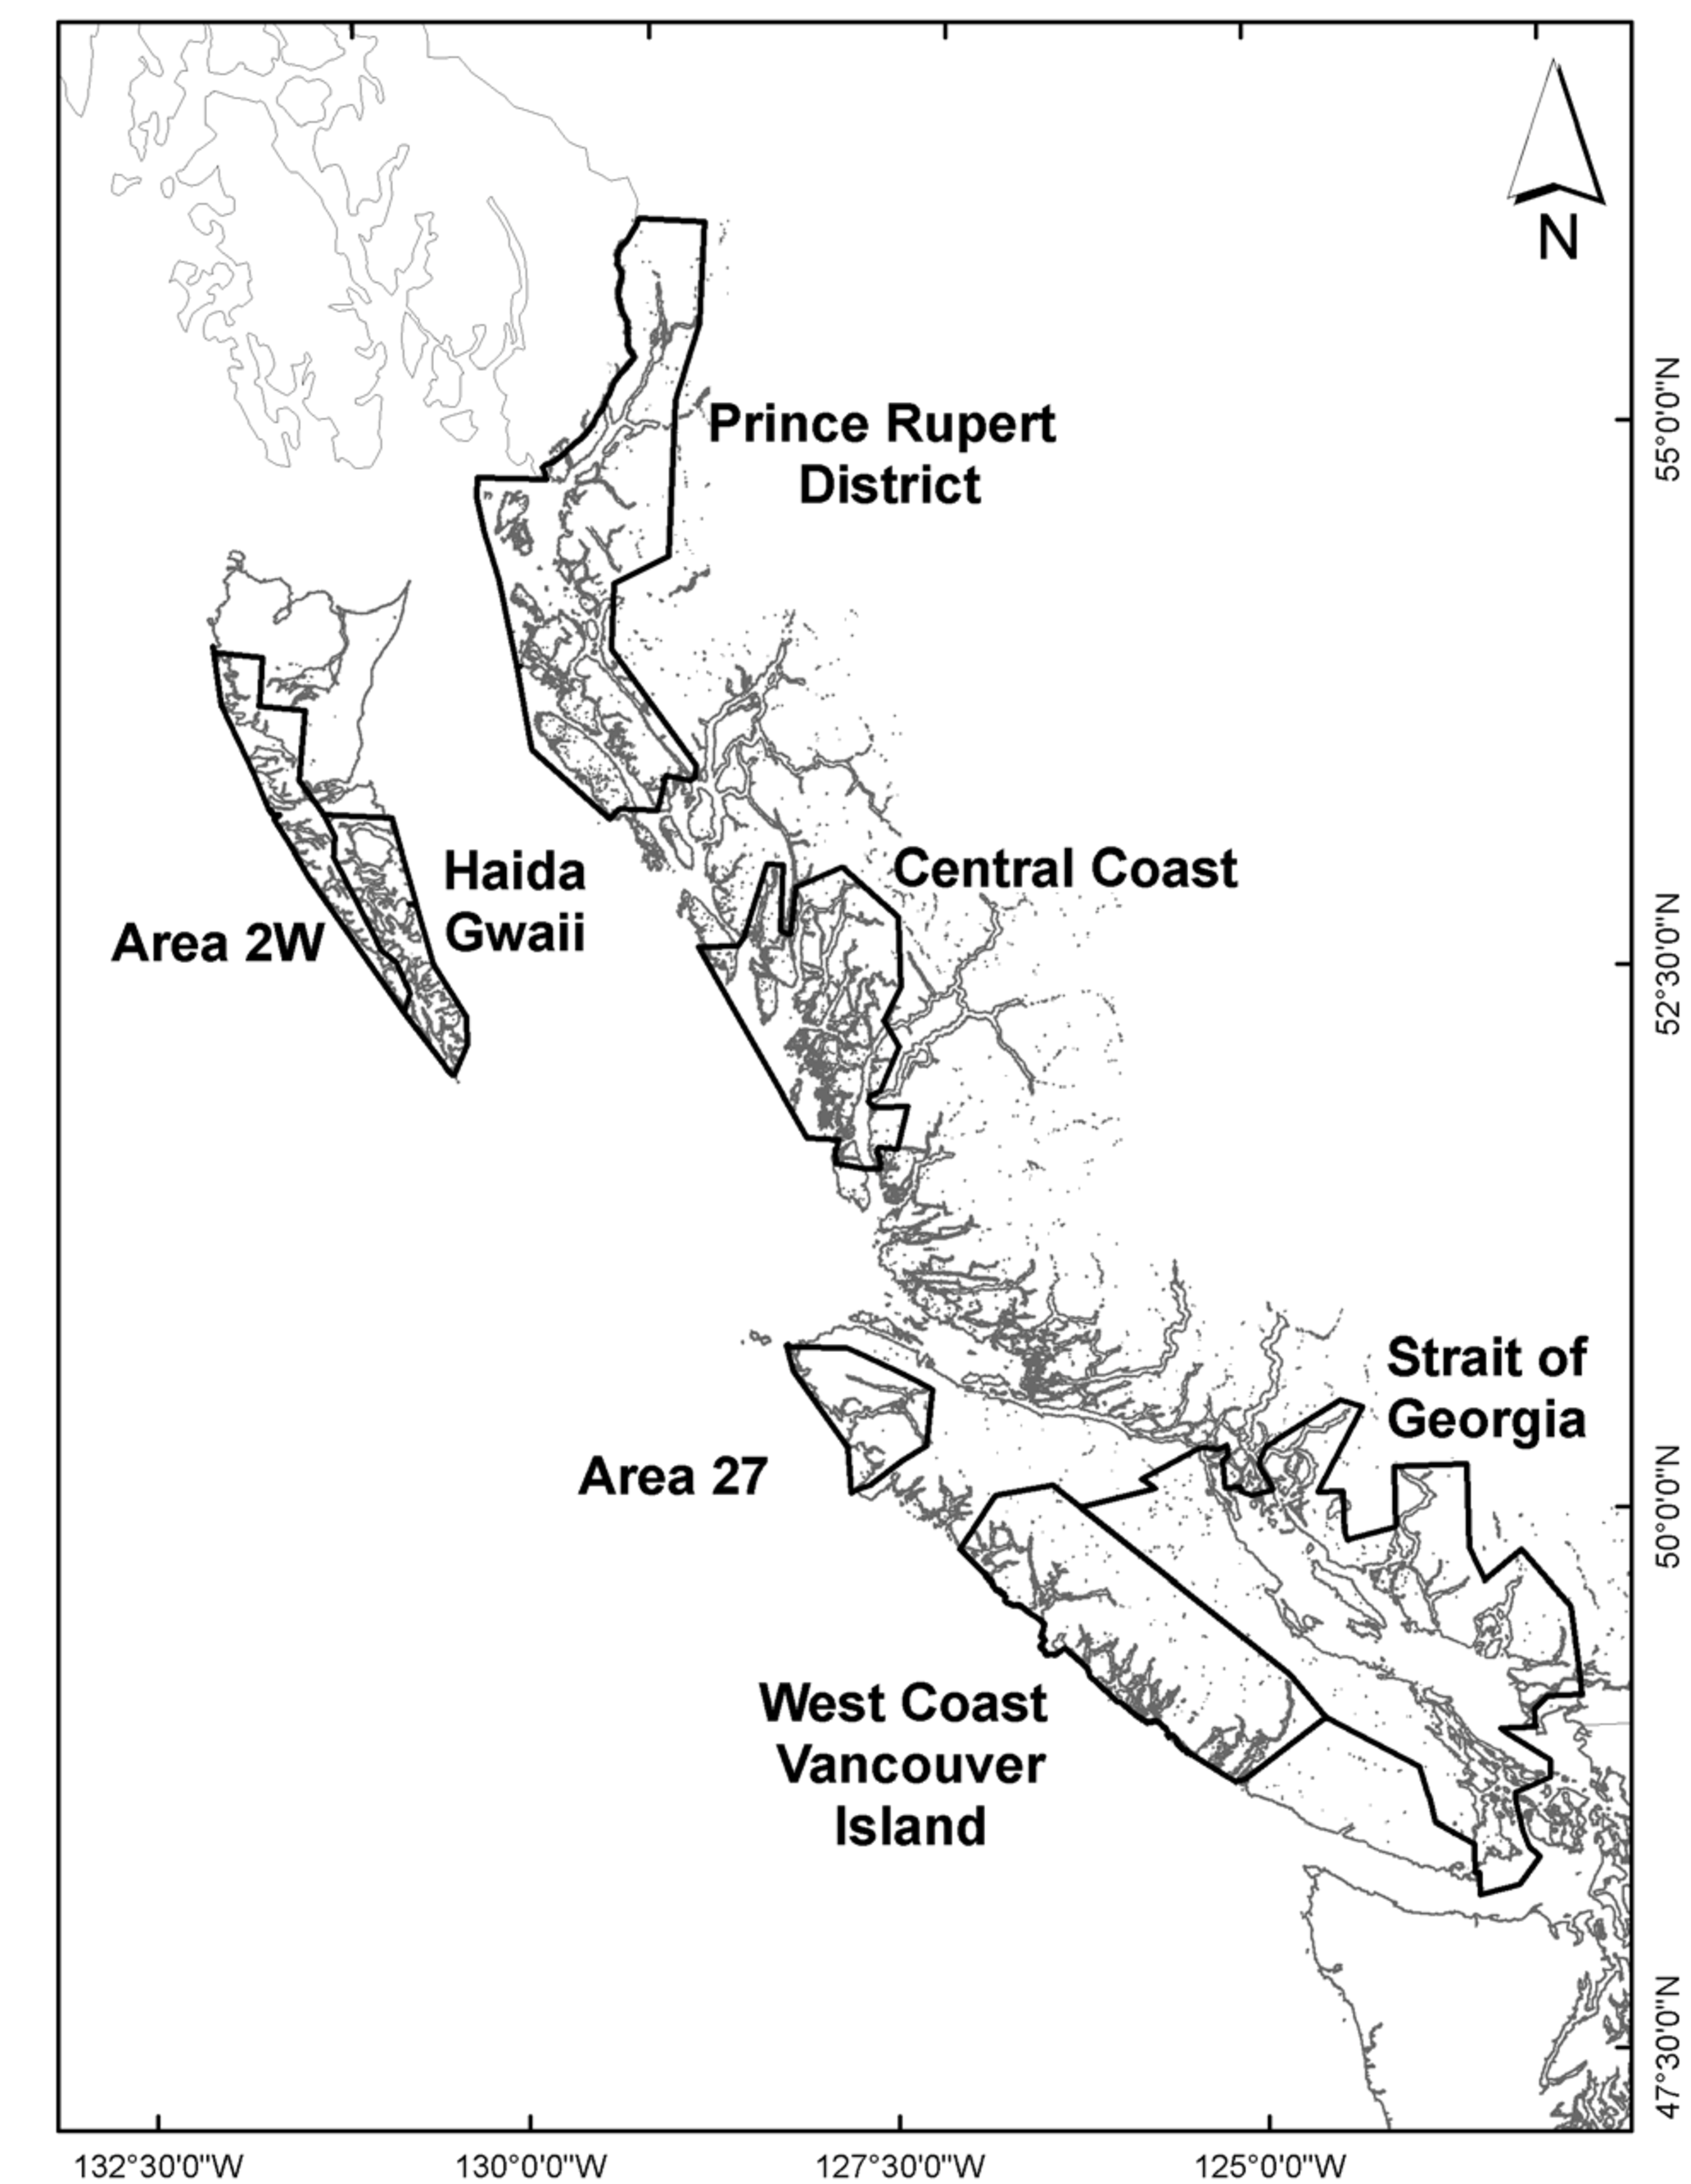
\includegraphics[width=\textwidth]{Figs/HerringAreaMap.pdf}
	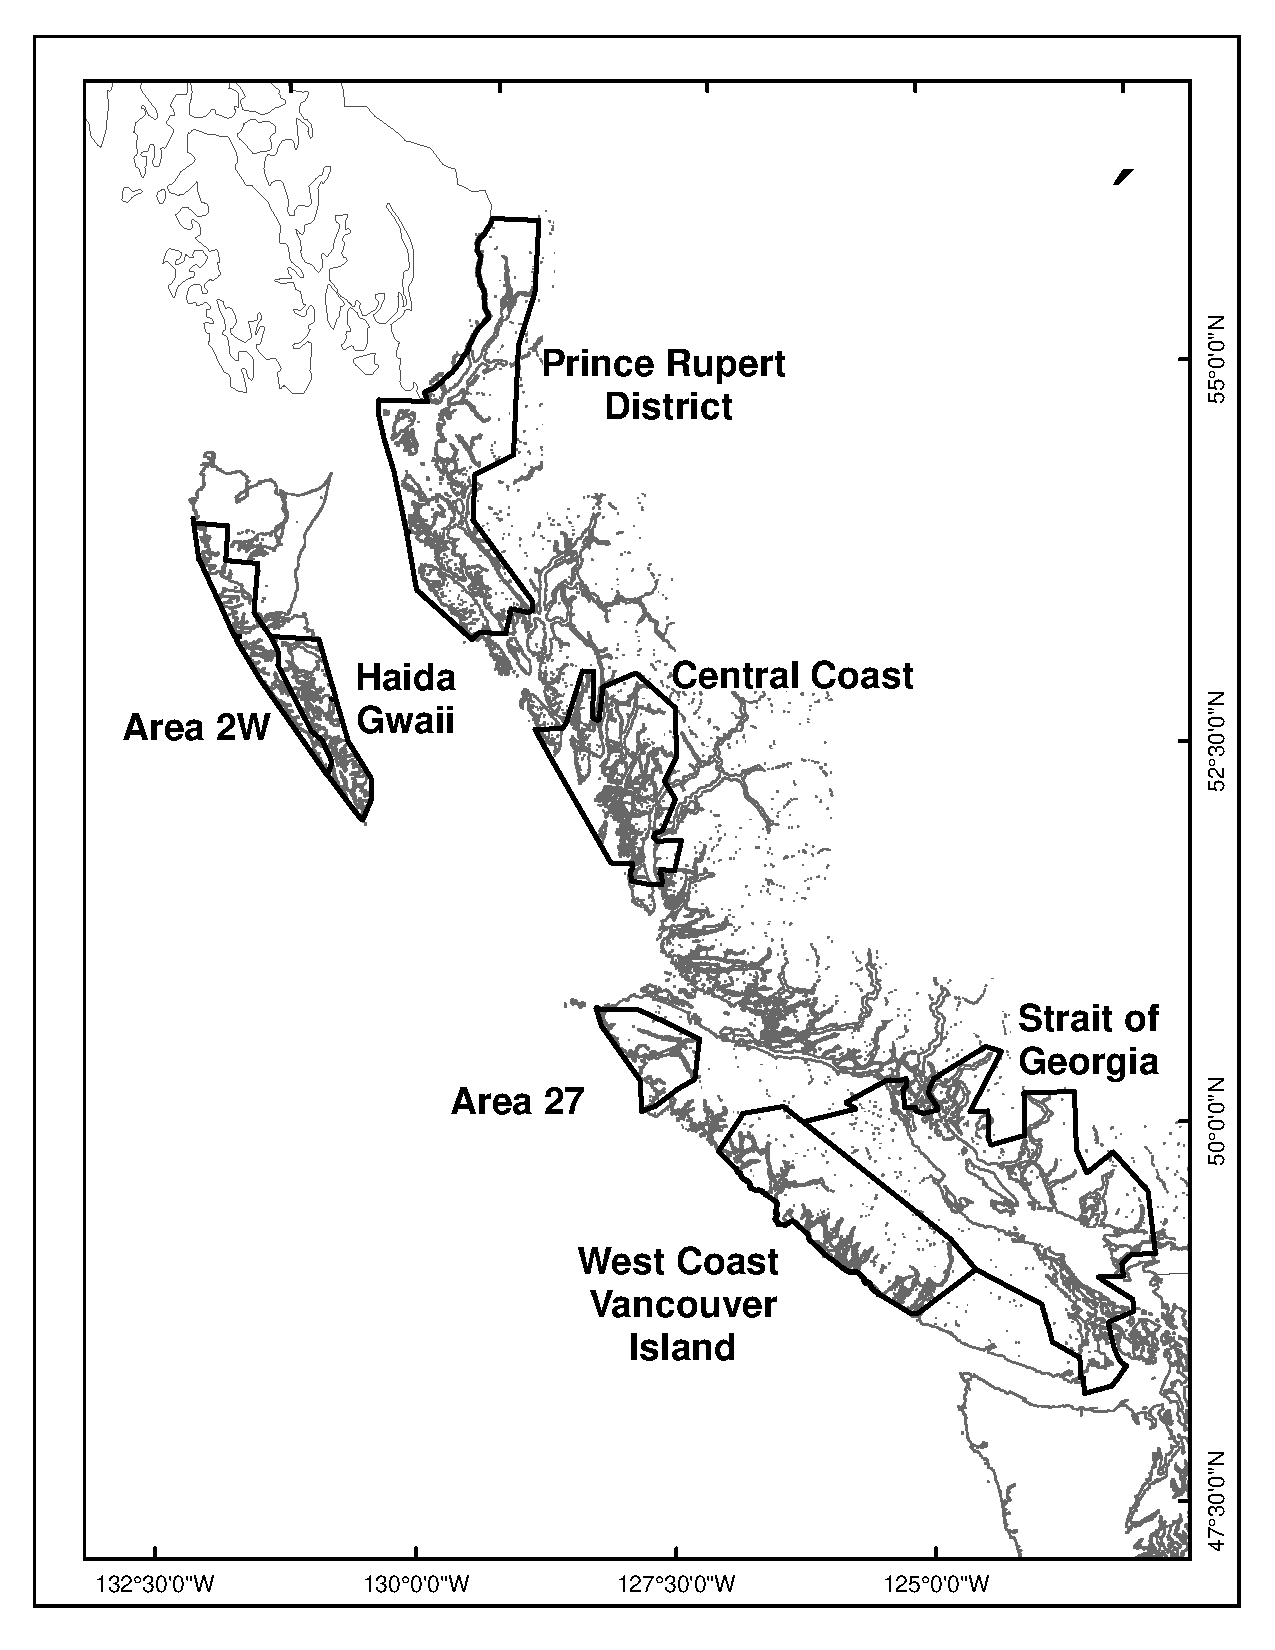
\includegraphics[width=0.95\textwidth]{../FIGS/PBSfigs/Assessment_Regions_2W_27_2010_HG.pdf}
	\caption{B.C. herring major stock areas: Haida Gwaii (HG or QCI 2E), Prince Rupert District (PRD), Central
Coast (CC), Strait of Georgia (SOG), West Coast Vancouver Island (WCVI), and minor stock areas: Area 2W and
Area 27.}\label{II:fig:map}
\end{figure}